\section{Implementation}
\label{sec:implementation}

We have implemented the NDN-IoT framework and a prototype of the Flow entertainment experience to verify the design introduced in the previous section.
The implementation follows a modular structure and differentiates between the framework-level services that we believe are common to many home IoT systems and the functionality that supports Flow-specific application logic.
This section describes details in both the framework and application components.

\subsection{NDN-IoT framework}

The NDN-IoT framework includes an implementation of the authentication server and a set of client libraries.

% AS
The AS functionality is implemented based on the team's previous work on NDN-pi (citation: ndn-pi TR).
The framework provides a server implementation in Python, which we run on Raspbian platform in Flow application.
The server implementation also updates the codebase to work with PyNDN2 2.0b4, with major updates to security module interface, including using CCL library's built-in public/private key storages. \footnote{We now use BasicIdentityStorage and FilePrivateKeyStorage for key storage, and ConfigPolicyManager for data verification, whereas the old implementation, developed at a time when PyNDN security library module was evolving, used custom derived classes (for example, IotPrivateKeyStorage).}
Authentication clients are available in both Python and JavaScript in order to support application components running on Ubuntu, OSX, Raspbian, and browser (Chrome and Firefox) platforms.
Compared with the earlier work in NDN-pi, this implementation added a port in JavaScript to support browser applications. 
The JavaScript port uses the library's IndexedDbIdentityStorage and IndexedDbPrivateKeyStorage for key storage (this means the key storage in browser is origin-based, thus in our installation the webpage that adds this ``device'' and the webpage that publishes application content should be hosted under the same origin). 
Recall that in NDN-pi the client device generates a device ID\footnote{The server uses this ID to construct the initial ``add device'' interest name. This ID was implemented as the CPU serial of a Raspberry Pi.}. 
In browser application's case we generate a random string in IndexedDB if one doesn't already exist, to use as the device identification of the device that currently runs the browser.

% NDN-IoT client libraries
The NDN-IoT client libraries are built on top of the NDN Common Client Libraries~\cite{ccl}, and aims to provide abstractions to faciliate application development in a home environment. 
The client libraries are available in Python, C++, JavaScript and C\#. 
They are organized into three major functional blocks:

\textbf{Bootstrap} follows the suggestion in section VI.B and VI.C of the IoTDI '16 paper, and helps with device and application identity setup. Its abstractions include: 
\begin{enumerate}
\item KeyChain setup: given a device identity (and optionally an AS name), construct a KeyChain and set up the default device certificate name for this application instance. This KeyChain is later used for signing and verification of all application data.
\item Consumer setup: given an application prefix, the Bootstrap module keeps outstanding interest for the application's trust schema (add example), and updates the local copy whenever a later version is received and verified.\footnote{The application trust schema may evolve over time, when new device names are added and authorized to publish under certain application prefixes}
\item Producer setup: given an application prefix, the Bootstrap module requests authorization from the AS to publish under that prefix by sending a command interest including this device's identity and the prefix it wants to publish for (add example). If the AS authorizes the request, it adds an entry stating to the application trust schema to reflect the updated trust relationship, and publishes a new version for all consumers to fetch.
\end{enumerate}

In practice, the application code to set up a gyroscope data producer on a Raspberry Pi may look like the following.
\begin{minted}
[frame=lines,
framesep=2mm,
baselinestretch=1,
fontsize=\footnotesize,
breaklines
]{python}
from ndn_iot_python import Bootstrap
deviceName = Name("/AliceHome/devices/rpi2")
dataPrefix = Name("/AliceHome/flow1/gyros")
appName = "flow1"
face = Face()
bootstrap = Bootstrap(face)
bootstrap.setupDefaultIdentityAndRoot(deviceName, onSetupComplete, onSetupFailed)

def onSetupComplete(certificateName, keyChain)
  bootstrap.requestProducerAuthorization(dataPrefix, appName, onRequestSuccess, onRequestFailed)

def onSetupFailed(message)
  print(message)
\end{minted}

And in a Flow application instance ``flow1'', a trust schema built by the AS may contain the following sections.
\begin{minted}[frame=lines,
framesep=2mm,
baselinestretch=1,
fontsize=\footnotesize,
breaklines
]{text}
trust-anchor 
{
  type "base64"
  base64-string "Bv0DD..."
}
\end{minted}
Trust anchor certificate is installed during the bootstrap process.
This rule is automatically populated by the AS.

\begin{minted}[frame=lines,
framesep=2mm,
baselinestretch=1,
fontsize=\footnotesize,
breaklines
]{text}
rule 
{
  id "Certs"
  for "data"
  filter 
  {
    type "regex"
    regex "^[^<KEY>]*<KEY><>*<ID-CERT>"
  }
  checker 
  {
    type "customized"
    sig-type "rsa-sha256"
    key-locator 
    {
      type "name"
      name "/AliceHome/devices/gateway/KEY/ksk
-1485314801/ID-CERT"
      relation "equal"
    }
  }
}
\end{minted}
This rule mandates that all certificates should be signed by the gateway.\footnote{In this iteration of Flow, device certicates are the only type of certificate involved in the trust relationship in Section~\ref{sec:trust-management}.}
This rule is automatically populated by the AS.

\begin{minted}[frame=lines,
framesep=2mm,
baselinestretch=1,
fontsize=\footnotesize,
breaklines
]{text}
rule 
{
  id "discovery-data"
  for "data"
  filter 
  {
    type "regex"
    regex "^[^<discovery>]*<discovery><>*"
  }
  checker 
  {
    type "customized"
    sig-type "rsa-sha256"
    key-locator 
    {
      type "name"
      regex "^[^<KEY>]*<KEY><>*<ID-CERT>"
    }
  }
}
\end{minted}
This rule mandates that all discovery data should be signed. 
This rule is automatically populated by the AS.

\begin{minted}[frame=lines,
framesep=2mm,
baselinestretch=1,
fontsize=\footnotesize,
breaklines
]{text}
rule 
{
  id "/AliceHome/flow1/gyros"
  for "data"
  filter 
  {
    type "name"
    name "/AliceHome/flow1/gyros"
    relation "is-prefix-of"
  }
  checker 
  {
    type "customized"
    sig-type "rsa-sha256"
    key-locator 
    {
      type "name"
      name "/AliceHome/devices/rpi2/KEY/dsk-
1485374576/ID-CERT"
      relation "equal"
    }
  }
}
\end{minted}
This rule mandates that data under application prefix \ndnName{/AliceHome/flow1/gyros} should be signed by device \ndnName{/AliceHome/devices/rpi2}.
This rule is added to the trust schema after the AS approves the request from \ndnName{/AliceHome/devices/rpi2}.

\textbf{Discovery} uses a simple sync-based discovery similar to ChronoSync recovery mechanism.

In practice, after setting up the Bootstrap object, the application may use the following code to include a discovery module.
\begin{minted}[frame=lines,
framesep=2mm,
baselinestretch=1,
fontsize=\footnotesize,
breaklines
]{python}
from ndn_iot_python import Discovery, Observer

class MyObserver(Observer):
  def onDiscovered(name, description):
    print(name.toUri() + description)

keyChain = bootstrap.getKeyChain()
certName = bootstrap.getDefaultCertificateName()
syncPrefix = Name("/AliceHome/discovery")
discovery = Discovery(face, keyChain, certName, syncPrefix, MyObserver())

description = "My Raspberry Pi device"
deviceName = Name("/home/devices/rpi2")
discovery.publishObject(deviceName, description)
\end{minted}

\textbf{Application-level pub/sub} follows the suggestion in section VI.F of the IoTDI '16 paper, and provides the following abstractions:
\begin{enumerate}
\item Consumer for timestamp namespace (/prefix/[timestamp]): this consumer uses oustanding interest with range exclusion to ask for latest piece of data, and upon data retrieval and successful verification, updates the range exclusion with the received timestamp.
\item Consumer for sequence-number namespace (/prefix/[sequence-number]): this consumer pipelines interest for the next few sequence numbers, and upon data retrieval and successful verification, issues an interest for the sequence number after the last one in the pipeline.
\end{enumerate}

In practice, after setting up the Bootstrap object, the application may use the following code to include a sequence number consumer module.

\begin{minted}[frame=lines,
framesep=2mm,
baselinestretch=1,
fontsize=\footnotesize,
breaklines
]{python}
from ndn_iot_python import AppConsumerSequenceNumber
keyChain = bootstrap.getKeyChain()
pipelineSize = 5
consumer = AppConsumerSequenceNumber(face, keyChain, pipelineSize)
prefix = Name("/home/flow1/gyros")
consumer.consume(prefix, onData, onTimeout, onVerifyFailed)
\end{minted}

\subsection{Flow application components}

% Subsystems
In our application prototype, each of the components is implemented as the following:
\begin{enumerate}
\item \textit{Indoor positioning}: We use OpenPTrack,\footnote{\url{http://openptrack.org/about/}} a multi-camera person tracking system.
The NDN producer for OpenPTrack\footnote{\url{https://github.com/OpenPTrack/ndn-opt/}} (written in C++)  publishes the position of each person at a 30Hz rate, along with lower rate metadata about active tracks. 
% Interest pipelining and an application-level Pending Interest Table are used for real-time delivery of position data.
% Dealing with constrained devices: better in design or implementation? deserve its own paragraph and figure?
\item \textit{Wearable sensing}: We use an RFduino 22301 with gyroscope MPU6050 attached to provide virtual camera control. 
The RFduino cannot perform asynchronous signing operations quickly enough, so we introduced a Raspberry Pi controller as a gateway for bridging RFduino to the NDN home network.
The data exchanged between RFduino and Raspberry Pi is signed with a shared secret key negotiated after Bluetooth pairing.
The Raspberry Pi generates a public/private key pair on behalf of the RFduino to be associated with the RFduino's device identity.
The RFduino runs a minimum NDN producer, implemented with the ndn-cpp-lite library\footnote{\url{https://github.com/named-data/ndn-cpp/}}, which generates data at roughly 2Hz rate.
When new data is generated, the RFduino pushes the data (signed by the pre-negotiated shared secret) to the Raspberry Pi controller over the Bluetooth LE channel.
The controller receives the data, repackages the data and signs the data using RFduino's private key, and then publishes the data on the home network.
The RFduino data publishing process is shown in Fig.~\ref{fig:contrained-devices-bootstrap}.
% More reasons needed for matching between IDs?
\item \textit{Mobile phone interface}: We employ an Android phone that loads a control webpage (written in JavaScript) in a mobile browser to interact with the virtual environment. 
The phone sends out two types of command Interests: the first one matches an OpenPTrack track ID with that of the mobile, and the second one drops an image onto the virtual environment where the user's avatar is standing. ID matching is introduced so that the visualization knows the location of the user's avatar (identified by a track ID) when an image drop command Interest is issued by the same user (identified by the mobile's ID).
\item \textit{Visualization}: We use the Unity3D\footnote{\url{https://unity3d.com}} game engine for visualization.
The game engine runs C\# NDN data consumers that receive person tracking and virtual camera control data, and a producer that receives image dropping command Interests from the mobile web interface.
\end{enumerate}

\begin{figure}[!t]
\centering
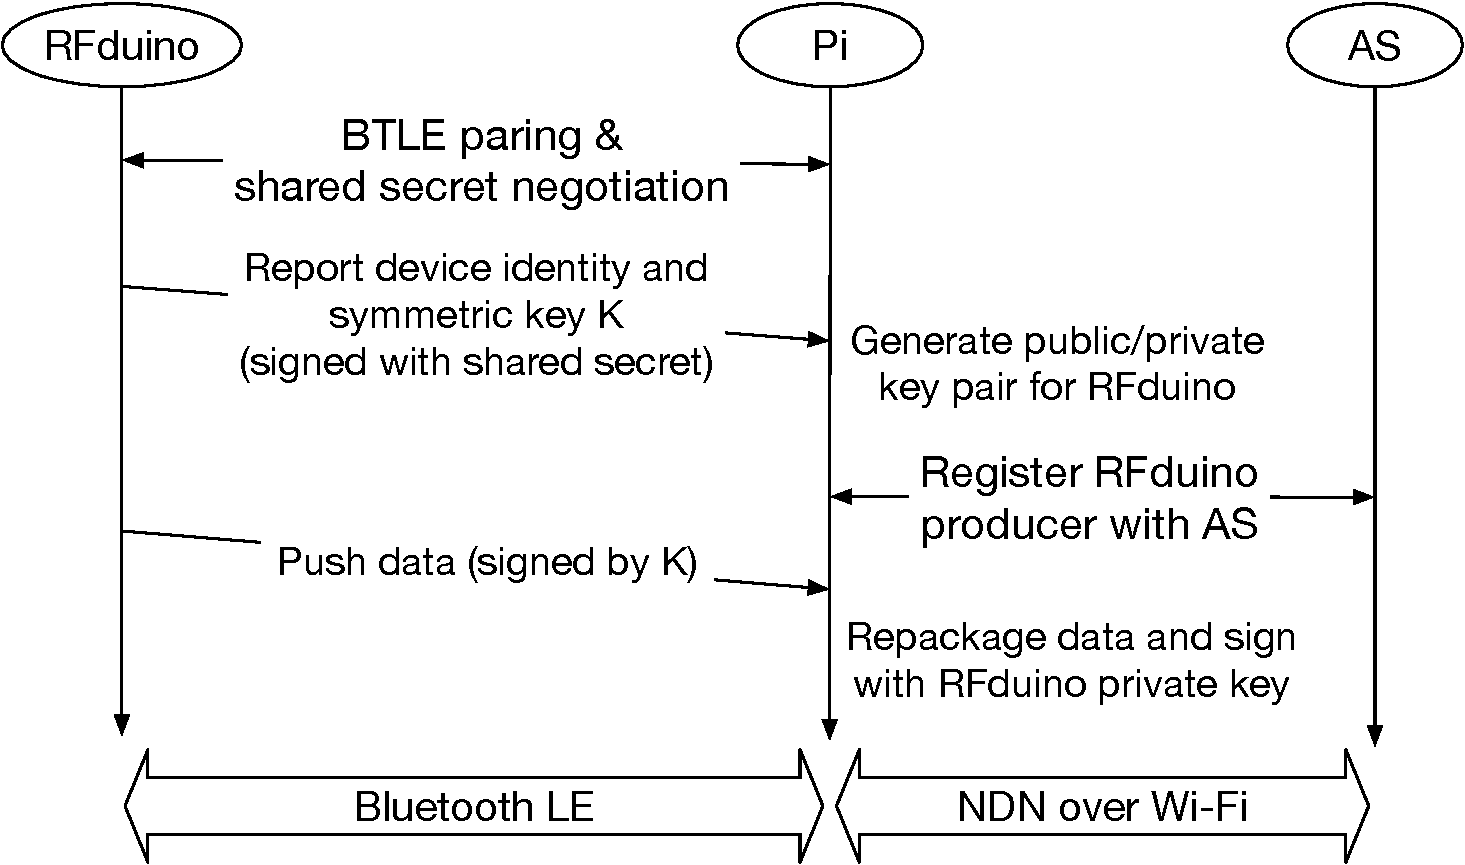
\includegraphics[width=0.95\columnwidth]{constrained-device-authorization.pdf}
\caption{RFduino data publishing with assistance of Raspberry Pi controller}
\label{fig:contrained-devices-bootstrap}
\end{figure}

The implementation for both NDN-IoT framework and Flow application are available online.\footnote{\url{https://github.com/remap/ndn-flow}} We installed two instances of the Flow application testbed at UCLA and Huawei. Fig.~\ref{fig:message-flow-in-flow-installation} shows a diagram of the system and its message flows after all devices are bootstrapped with an AS, which in our installation is another Raspberry Pi.

\begin{figure*}[!t]
\centering
\includegraphics[width=0.95\textwidth]{flow-components-ndn-names-diagram-zs.pdf}
\caption{Application components and message flows in Flow}
\label{fig:message-flow-in-flow-installation}
\end{figure*}
